\documentclass{standalone}

%----------------------------------------------------------------------------------------------%
%                                 Packages and basic declarations
%----------------------------------------------------------------------------------------------%

\usepackage{verbatim}
\usepackage{pgf}
\usepackage{tikz}
\usepackage{mathrsfs}

\usetikzlibrary{arrows}

%----------------------------------------------------------------------------------------------%
%----------------------------------------------------------------------------------------------%
%                                            DOCUMENT STARTS
%----------------------------------------------------------------------------------------------%
%----------------------------------------------------------------------------------------------%

\begin{document}

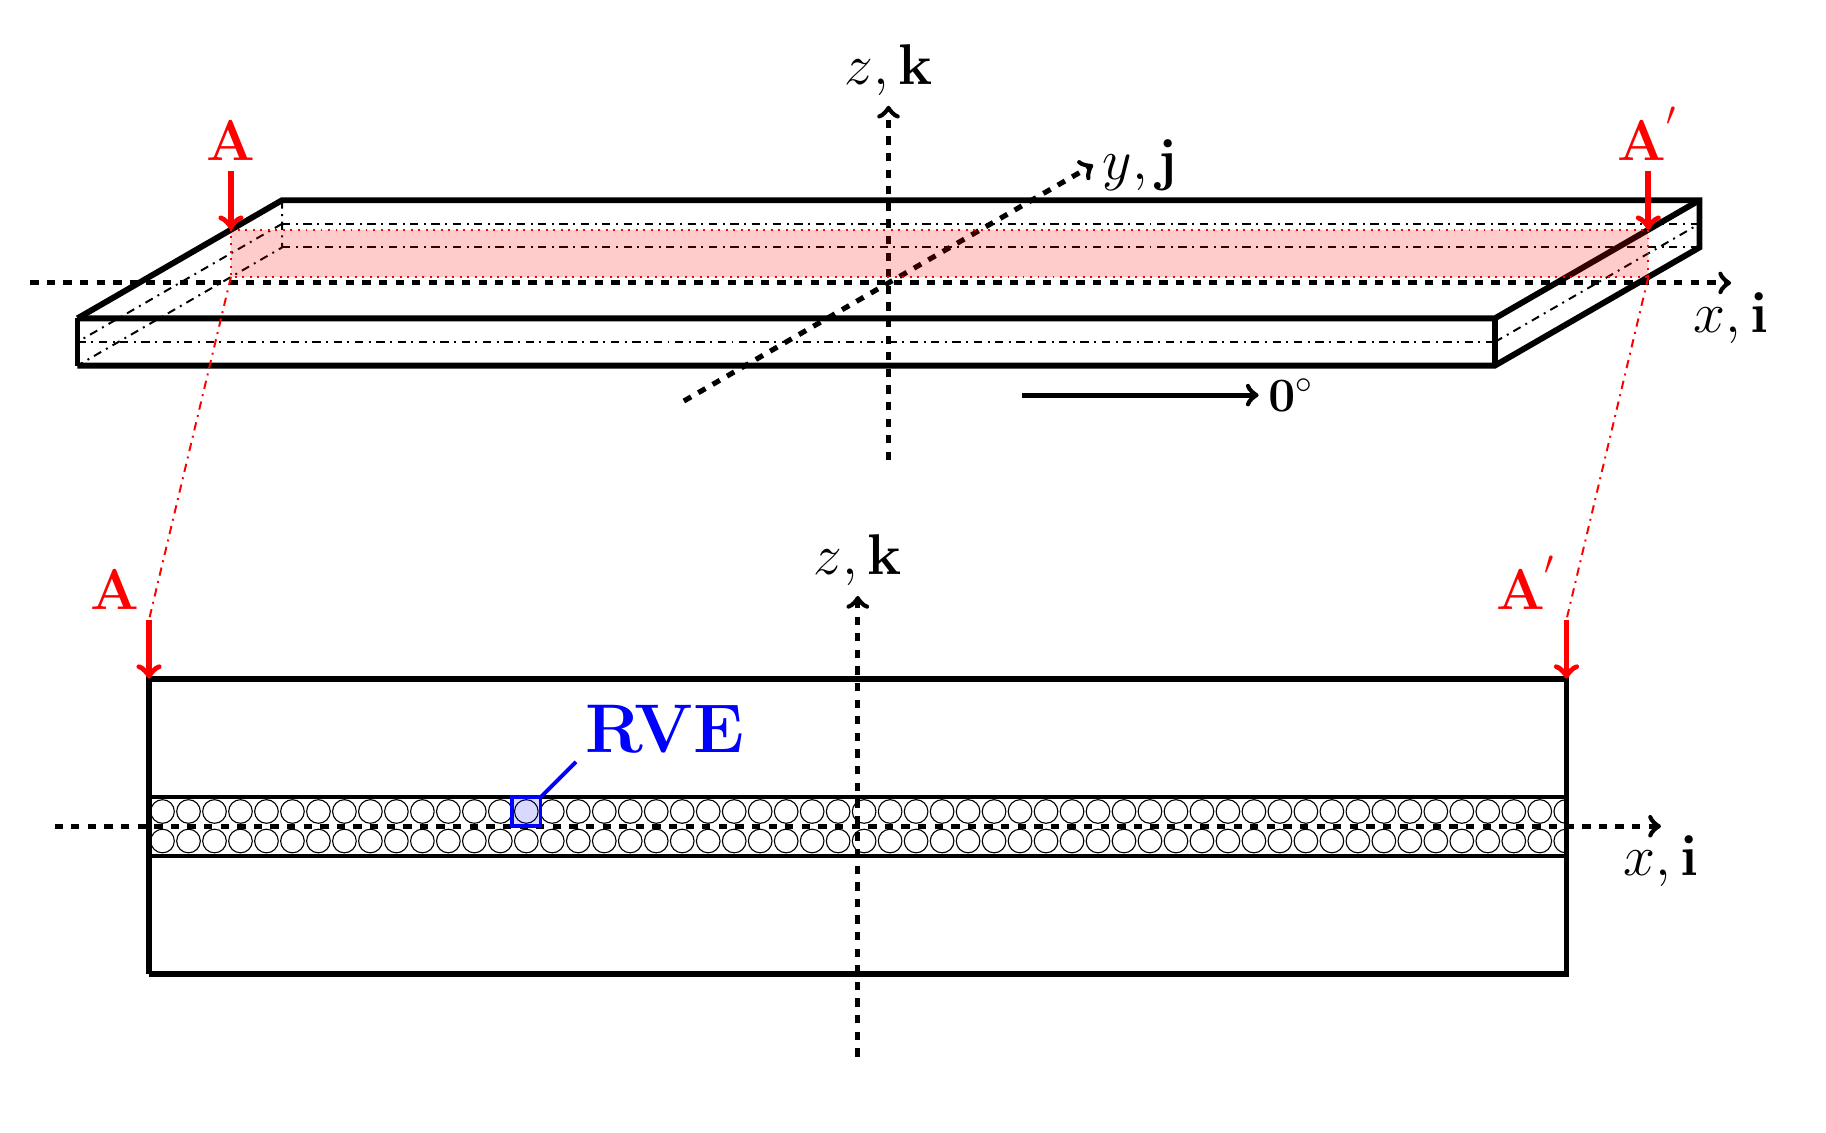
\begin{tikzpicture}[scale=1.5]
%[scale=4.5,cap=round,x=1cm,y=1cm]

%----------------------------------------------------------------------------------------------%
%                                          INPUT PARAMETERS
%----------------------------------------------------------------------------------------------%

\def\Rf{0.1}
\def\l{10}

%----------------------------------------------------------------------------------------------%
%                                        COMMAND DEFINITION
%----------------------------------------------------------------------------------------------%

\newcommand{\refSystem}[9]{

	\def\xO{#1}
	\def\xlow{#2}
	\def\xup{#3}
	\def\zO{#4}
	\def\zlow{#5}
	\def\zup{#6}
	\def\ylow{#7}
	\def\yup{#8}


	\pgfmathsetmacro\cosphi{cos(30)}
	\pgfmathsetmacro\sinphi{sin(30)}

	\tikzstyle{axes}=[]

	\begin{scope}[style=axes]
 		\draw[->,draw=#9] (\xO-\xlow,0) -- (\xO+\xup,0) ;
 		\draw[->,draw=#9] (0,\zO-\zup) -- (0,\zO+\zup) ;
		\draw[->,draw=#9] (\xO-\ylow*\cosphi,\zO-\ylow*\sinphi) --(\xO+\yup*\cosphi,\zO+\yup*\sinphi) ;
		\node[anchor=north] at (\xO+\xup,0) {$x,\mathbf{i}$};
		\node[anchor=west] at (\xO+\yup*\cosphi,\zO+\yup*\sinphi) {$y,\mathbf{j}$};
		\node[anchor=west] at (0,\zO+\zup) {$z,\mathbf{k}$};
	\end{scope}
}

\newcommand{\drawFiber}[6]{
	%#1 -> Rf
	%#2 -> theta
	%#3 -> deltatheta
	%#4 -> line color
	%#5 -> x0
	%#6 -> y0

	\def\R{#1}
	\def\thetavalue{#2}
	\def\dtheta{#3}
	\def\x{#5}
	\def\y{#6}

	\pgfmathsetmacro\costhetaup{cos(\thetavalue+\dtheta)}
	\pgfmathsetmacro\sinthetaup{sin(\thetavalue+\dtheta)}

	\pgfmathsetmacro\costhetabot{cos(\thetavalue-\dtheta)}
	\pgfmathsetmacro\sinthetabot{sin(\thetavalue-\dtheta)}

	\def\thetaround{360+\thetavalue-\dtheta}

	%draw fiber surface
	\draw[draw=#4] (\x+\R*\costhetaup,\y+\R*\sinthetaup)arc (\thetavalue+\dtheta:\thetaround:\R);
	%draw radius
	%\draw[dashed](0,0)--(-\costhetabot,\sinthetabot);

}

\pgfmathsetmacro\cosproj{cos(30)}
\pgfmathsetmacro\sinproj{sin(30)}

\draw[->,draw=black,dashed,line width=0.65mm] (-32*2*\Rf,10*\Rf*\sinproj) -- (40*2*\Rf,10*\Rf*\sinproj) ;
\draw[->,draw=black,dashed,line width=0.65mm] (10*\Rf*\cosproj,10*\Rf*\sinproj-15*\Rf) -- (10*\Rf*\cosproj,10*\Rf*\sinproj+15*\Rf) ;
\draw[->,draw=black,dashed,line width=0.65mm] (-10*\Rf*\cosproj,-10*\Rf*\sinproj) -- (30*\Rf*\cosproj,30*\Rf*\sinproj) ;
\node[anchor=north] at (40*2*\Rf,10*\Rf*\sinproj) {\huge $x,\mathbf{i}$};
\node[anchor=west] at (30*\Rf*\cosproj,30*\Rf*\sinproj) {\huge $y,\mathbf{j}$};
\node[anchor=south] at (10*\Rf*\cosproj,10*\Rf*\sinproj+15*\Rf)  {\huge $z,\mathbf{k}$};

\draw[line width=0.75mm] (-30*2*\Rf,-2*\Rf) -- (30*2*\Rf,-2*\Rf) --  (30*2*\Rf+20*\Rf*\cosproj,-2*\Rf+20*\Rf*\sinproj)  -- (30*2*\Rf+20*\Rf*\cosproj,2*\Rf+20*\Rf*\sinproj) -- (-30*2*\Rf+20*\Rf*\cosproj,2*\Rf+20*\Rf*\sinproj) -- (-30*2*\Rf,2*\Rf);
\draw[line width=0.75mm](-30*2*\Rf,2*\Rf) -- (30*2*\Rf,2*\Rf) --  (30*2*\Rf+20*\Rf*\cosproj,2*\Rf+20*\Rf*\sinproj);
\draw[line width=0.75mm](-30*2*\Rf,-2*\Rf) -- (-30*2*\Rf,2*\Rf) ;
\draw[line width=0.75mm](30*2*\Rf,-2*\Rf) -- (30*2*\Rf,2*\Rf) ;
\draw[line width=0.25mm,dash dot](-30*2*\Rf+20*\Rf*\cosproj,2*\Rf+20*\Rf*\sinproj) -- (-30*2*\Rf+20*\Rf*\cosproj,-2*\Rf+20*\Rf*\sinproj) -- (-30*2*\Rf,-2*\Rf);
\draw[line width=0.25mm,dash dot](-30*2*\Rf+20*\Rf*\cosproj,-2*\Rf+20*\Rf*\sinproj) --  (30*2*\Rf+20*\Rf*\cosproj,-2*\Rf+20*\Rf*\sinproj);
\draw[line width=0.25mm,dash dot](-30*2*\Rf,0.) --  (30*2*\Rf,0.);
\draw[line width=0.25mm,dash dot] (30*2*\Rf,0) --  (30*2*\Rf+20*\Rf*\cosproj,0+20*\Rf*\sinproj);
\draw[line width=0.25mm,dash dot](-30*2*\Rf+20*\Rf*\cosproj,0+20*\Rf*\sinproj)  -- (30*2*\Rf+20*\Rf*\cosproj,0+20*\Rf*\sinproj);
\draw[line width=0.25mm,dash dot] (-30*2*\Rf+20*\Rf*\cosproj,0+20*\Rf*\sinproj) -- (-30*2*\Rf,0);

\draw[line width=0.25mm,dotted,draw=red, fill=red, fill opacity=0.2](30*2*\Rf+15*\Rf*\cosproj,-2*\Rf+15*\Rf*\sinproj) -- (30*2*\Rf+15*\Rf*\cosproj,2*\Rf+15*\Rf*\sinproj) -- (-30*2*\Rf+15*\Rf*\cosproj,2*\Rf+15*\Rf*\sinproj) -- (-30*2*\Rf+15*\Rf*\cosproj,-2*\Rf+15*\Rf*\sinproj) -- (30*2*\Rf+15*\Rf*\cosproj,-2*\Rf+15*\Rf*\sinproj);

\draw[->,line width=0.75mm,draw=red](30*2*\Rf+15*\Rf*\cosproj,7*\Rf+15*\Rf*\sinproj)--(30*2*\Rf+15*\Rf*\cosproj,2*\Rf+15*\Rf*\sinproj);
\draw[->,line width=0.75mm,draw=red](-30*2*\Rf+15*\Rf*\cosproj,7*\Rf+15*\Rf*\sinproj)--(-30*2*\Rf+15*\Rf*\cosproj,2*\Rf+15*\Rf*\sinproj);
\node[anchor=south, text=red] at (30*2*\Rf+15*\Rf*\cosproj,7*\Rf+15*\Rf*\sinproj) {\huge $\mathbf{A^{'}}$};
\node[anchor=south, text=red] at (-30*2*\Rf+15*\Rf*\cosproj,7*\Rf+15*\Rf*\sinproj) {\huge $\mathbf{A}$};

\draw[->,draw=black,line width=0.65mm] (10*2*\Rf,-9*\Rf*\sinproj) -- (20*2*\Rf,-9*\Rf*\sinproj) ;
\node[anchor=west, text=black] at (20*2*\Rf,-9*\Rf*\sinproj) {\LARGE $\mathbf{0^{\circ}}$};


\node[anchor=west] at (42*2*\Rf,10*\Rf*\sinproj) { };
\node[anchor=south] at (0,25*\Rf) {};
\node[anchor=north] at (0, -63*\Rf) {};


\pgfmathsetmacro\transl{30*\Rf}

\draw[line width=0.25mm,dash dot,draw=red](30*2*\Rf+15*\Rf*\cosproj,-2*\Rf+15*\Rf*\sinproj) --  (30*2*\Rf+7*\Rf*\cosproj,3*\Rf+7*\Rf*\sinproj-\transl);
\draw[line width=0.25mm,dash dot,draw=red](-30*2*\Rf+15*\Rf*\cosproj,-2*\Rf+15*\Rf*\sinproj) -- (-30*2*\Rf+7*\Rf*\cosproj,3*\Rf+7*\Rf*\sinproj-\transl);

\draw[line width=0.75mm]  (-30*2*\Rf+7*\Rf*\cosproj,-2*\Rf+7*\Rf*\sinproj-25*\Rf-\transl) -- (-30*2*\Rf+7*\Rf*\cosproj,-2*\Rf+7*\Rf*\sinproj-\transl) -- (30*2*\Rf+7*\Rf*\cosproj,-2*\Rf+7*\Rf*\sinproj-\transl) -- (30*2*\Rf+7*\Rf*\cosproj,-2*\Rf+7*\Rf*\sinproj-25*\Rf-\transl) -- (-30*2*\Rf+7*\Rf*\cosproj,-2*\Rf+7*\Rf*\sinproj-25*\Rf-\transl);

\draw[->,line width=0.75mm,draw=red](-30*2*\Rf+7*\Rf*\cosproj,3*\Rf+7*\Rf*\sinproj-\transl)--(-30*2*\Rf+7*\Rf*\cosproj,-2*\Rf+7*\Rf*\sinproj-\transl);
\draw[->,line width=0.75mm,draw=red](30*2*\Rf+7*\Rf*\cosproj,3*\Rf+7*\Rf*\sinproj-\transl)--(30*2*\Rf+7*\Rf*\cosproj,-2*\Rf+7*\Rf*\sinproj-\transl);
\node[anchor=south east, text=red] at (-30*2*\Rf+7*\Rf*\cosproj,3*\Rf+7*\Rf*\sinproj-\transl) {\huge $\mathbf{A}$};
\node[anchor=south east, text=red] at (30*2*\Rf+7*\Rf*\cosproj,3*\Rf+7*\Rf*\sinproj-\transl) {\huge $\mathbf{A^{'}}$};

\draw[->,draw=black,dashed,line width=0.65mm] (-34*2*\Rf+7*\Rf*\cosproj,-2*\Rf+7*\Rf*\sinproj-12.5*\Rf-\transl) -- (34*2*\Rf+7*\Rf*\cosproj,-2*\Rf+7*\Rf*\sinproj-12.5*\Rf-\transl);
\draw[->,draw=black,dashed,line width=0.65mm] (7*\Rf*\cosproj,-2*\Rf+7*\Rf*\sinproj-32*\Rf-\transl) -- (7*\Rf*\cosproj,-2*\Rf+7*\Rf*\sinproj+7*\Rf-\transl);
\node[anchor=north] at   (34*2*\Rf+7*\Rf*\cosproj,-2*\Rf+7*\Rf*\sinproj-12.5*\Rf-\transl) {\huge $x,\mathbf{i}$};
\node[anchor=south] at (7*\Rf*\cosproj,-2*\Rf+7*\Rf*\sinproj+7*\Rf-\transl)  {\huge $z,\mathbf{k}$};

\draw[line width=0.5mm](-30*2*\Rf+7*\Rf*\cosproj,-2*\Rf+7*\Rf*\sinproj-10*\Rf-\transl) -- (30*2*\Rf+7*\Rf*\cosproj,-2*\Rf+7*\Rf*\sinproj-10*\Rf-\transl);
\draw[line width=0.5mm](-30*2*\Rf+7*\Rf*\cosproj,-2*\Rf+7*\Rf*\sinproj-15*\Rf-\transl) -- (30*2*\Rf+7*\Rf*\cosproj,-2*\Rf+7*\Rf*\sinproj-15*\Rf-\transl);
\foreach \n in {-24,-23,-22,-21,-20,-19,-18,-17,-16,-15,-14,-13,-12,-11,-10,-9,-8,-7,-6,-5,-4,-3,-2,-1,0,1,2,3,4,5,6,7,8,9,10,11,12,13,14,15,16,17,18,19,20,21,22,23,24,25,26,27,28,29}{
	\drawFiber{\Rf}{0}{360}{black}{\n*2.2*\Rf}{-2*\Rf+7*\Rf*\sinproj-11.25*\Rf-\transl};
}
\drawFiber{\Rf}{0}{270}{black}{30*2.2*\Rf}{-2*\Rf+7*\Rf*\sinproj-11.25*\Rf-\transl};
\foreach \n in {-24,-23,-22,-21,-20,-19,-18,-17,-16,-15,-14,-13,-12,-11,-10,-9,-8,-7,-6,-5,-4,-3,-2,-1,0,1,2,3,4,5,6,7,8,9,10,11,12,13,14,15,16,17,18,19,20,21,22,23,24,25,26,27,28,29}{
	\drawFiber{\Rf}{0}{360}{black}{\n*2.2*\Rf}{-2*\Rf+7*\Rf*\sinproj-13.75*\Rf-\transl};
}
\drawFiber{\Rf}{0}{270}{black}{30*2.2*\Rf}{-2*\Rf+7*\Rf*\sinproj-13.75*\Rf-\transl};
\def\n{-10}
\draw[line width=0.5mm,draw=blue, fill=blue, fill opacity=0.15](\n*2.2*\Rf+1.2*\Rf,-2*\Rf+7*\Rf*\sinproj-11.25*\Rf-\transl+1.2*\Rf) -- (\n*2.2*\Rf+1.2*\Rf,-2*\Rf+7*\Rf*\sinproj-11.25*\Rf-\transl-1.2*\Rf) -- (\n*2.2*\Rf-1.2*\Rf,-2*\Rf+7*\Rf*\sinproj-11.25*\Rf-\transl-1.2*\Rf) -- (\n*2.2*\Rf-1.2*\Rf,-2*\Rf+7*\Rf*\sinproj-11.25*\Rf-\transl+1.2*\Rf) -- (\n*2.2*\Rf+1.2*\Rf,-2*\Rf+7*\Rf*\sinproj-11.25*\Rf-\transl+1.2*\Rf);

\draw[line width=0.5mm,draw=blue](\n*2.2*\Rf+1.2*\Rf,-2*\Rf+7*\Rf*\sinproj-11.25*\Rf-\transl+1.2*\Rf) -- (\n*2.2*\Rf+1.2*\Rf+3*\Rf,-2*\Rf+7*\Rf*\sinproj-11.25*\Rf-\transl+1.2*\Rf+3*\Rf);
\node[anchor=south west, text=blue] at (\n*2.2*\Rf+1.2*\Rf+3*\Rf,-2*\Rf+7*\Rf*\sinproj-11.25*\Rf-\transl+1.2*\Rf+3*\Rf) {\Huge \bf{RVE}};

%\node[rotate=90,anchor=south] at  (-34*2*\Rf,10*\Rf*\sinproj) {\Huge \bf{LAMINATE AS A 3D PLATE}};
%\node[rotate=90,anchor=south] at (-34*2*\Rf,-2*\Rf+7*\Rf*\sinproj-12.5*\Rf-\transl) {\Huge \bf{2D SECTION}};
%\node[rotate=90,anchor=south] at  (-36*2*\Rf,10*\Rf*\sinproj) {\LARGE };
%\node[rotate=90,anchor=south] at (-36*2*\Rf,-2*\Rf+7*\Rf*\sinproj-12.5*\Rf-\transl) {\LARGE };







\end{tikzpicture}

\end{document}
